\chapter{Evaluation Results}
\label{cha:evaluationResults}

In this chapter we present algorithm evaluation results and conclusions.

\section{Testing rig}

All algorithms were run on Lenovo W530 laptop with the following hardware and software:

\begin{itemize}
	\item CPU: Intel Core i7-3740QM (2.7 GHz)
	\item RAM size: 16 GB
	\item Operating system: Windows 7 Enterprise 64-bit
\end{itemize}

All tests were performed under "Maximum Performance" setting.

\section{Test data}

Numerous test cases were generated, varying in problem size, number of winners, generation model and satisfaction function.

\subsection{Problem size}

Problem size is defined by number of agents ($n$) and number of alternatives ($m$). We selected three problem sizes for testing:

\begin{itemize}
	\item Small instance: $n = 30$, $m = 10$
	\item Medium instance: $n = 400$, $m = 50$
	\item Large instance: $n = 400$, $m = 300$
\end{itemize}

\subsection{Number of winners}

For each problem size, we selected two different number of winners ($K$) - first one to take a small part of alternatives as winners (around 15-20\%) and the second one to take about half of alternatives as winners:
\begin{itemize}
	\item Small instance: $K = 2$ or $K = 5$
	\item Medium instance: $K = 10$ or $K = 25$
	\item Large instance: $K = 50$ or $K = 200$
\end{itemize}

\subsection{Data generation model}

Test data was generated using two different models.
\\

\noindent
\textbf{Polya urn model} (Polya) \hspace{.1in} This model assumes we have an urn with $m$ balls in $m$ colors, each representing an alternative. We generate preferences by drawing random balls from the urn. First, we draw alternatives for first rank in each agent's preference order, then for second ranks, and so on, until the entire preference profile is drawn. After the ball is drawn, it is returned to the urn and another ball of the same color is added to the urn too, so a probability of drawing the same color in the future is increased ("strong becomes stronger"). The only constraint is that an alternative cannot be drawn for an agent for which it has been already drawn before. This model generates preference profile where some relatively small number of alternatives is preferred to all the others by most agents.
\\

\noindent
\textbf{Impartial culture model} (IC) \hspace{.1in} In this model, for each agent we generate preference order independently. For each agent, every preference order (every permutation of alternatives) has equal probability of being drawn. This model generated preference profile with no clearly dominating alternatives.

\subsection{Satisfaction function}

Two different satisfaction functions were used, each of them trying to model real preferences of the voters.
\\

\noindent
\textbf{Square function} \hspace{.1in} This is simply a square function and it assumes that difference between voters in the first positions of the preference order should be higher than between the last positions (voter is more concerned with his favourite candidates, not the ones in the end of the list). The function is given as follows:

\begin{gather}
	\alpha(i) = (m - i)^{2}
\end{gather}
\\

Example of function for $m = 20$:

\begin{center}
	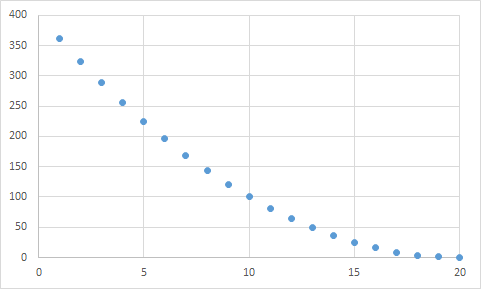
\includegraphics[scale=0.7]{satfun1}
\end{center}

\noindent
\textbf{Strange function} \hspace{.1in} This function assumes that for the voter the difference between two candidates from the top is the same as the difference between two candidates from the bottom, while differences between candidates from the middle of the preference order are much less significant. The function is given as follows:

\begin{gather}
	f(x) = \frac{n^{2}+n}{2} \\
	h = \frac{m}{2} \\
	d = f(h) \\
	\alpha(i) = \begin{cases} f(h-i+1)+d-1 : i<h \\ -f(i-h)+d : i \geq h \end{cases}
\end{gather}
\\

Example of function for $m = 20$:

\begin{center}
	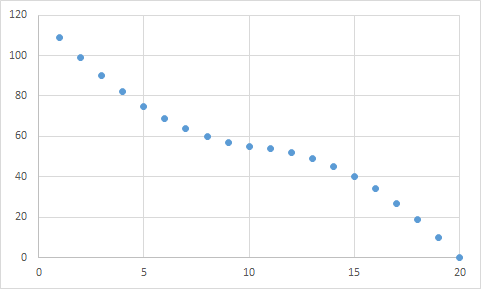
\includegraphics[scale=0.7]{satfun2}
\end{center}

\subsection{Summary}

Table below presents all generated test cases.

\begin{tabular}{r | c | c | c | c | c |}
	\# & alternatives count & agents count & winners count & genration model & satisfaction function \\
	\hline
	1 & \multirow{8}{*}{10} & \multirow{8}{*}{30} & \multirow{4}{*}{2} & \multirow{2}{*}{Polya} & Square \\
	2 & & & & & Strange \\
	\cline{5-6}
	3 & & & & \multirow{2}{*}{IC} & Square \\
	4 & & & & & Strange \\
	\cline{4-6}
	5 & & & \multirow{4}{*}{5} & \multirow{2}{*}{Polya} & Square \\
	6 & & & & & Strange \\
	\cline{5-6}
	7 & & & & \multirow{2}{*}{IC} & Square \\
	8 & & & & & Strange \\
	\hline
	9 & \multirow{8}{*}{50} & \multirow{8}{*}{400} & \multirow{4}{*}{10} & \multirow{2}{*}{Polya} & Square \\
	10 & & & & & Strange \\
	\cline{5-6}
	11 & & & & \multirow{2}{*}{IC} & Square \\
	12 & & & & & Strange \\
	\cline{4-6}
	13 & & & \multirow{4}{*}{25} & \multirow{2}{*}{Polya} & Square \\
	14 & & & & & Strange \\
	\cline{5-6}
	15 & & & & \multirow{2}{*}{IC} & Square \\
	16 & & & & & Strange \\
	\hline
	17 & \multirow{8}{*}{300} & \multirow{8}{*}{400} & \multirow{4}{*}{50} & \multirow{2}{*}{Polya} & Square \\
	18 & & & & & Strange \\
	\cline{5-6}
	19 & & & & \multirow{2}{*}{IC} & Square \\
	20 & & & & & Strange \\
	\cline{4-6}
	21 & & & \multirow{4}{*}{200} & \multirow{2}{*}{Polya} & Square \\
	22 & & & & & Strange \\
	\cline{5-6}
	23 & & & & \multirow{2}{*}{IC} & Square \\
	24 & & & & & Strange \\
	\hline
\end{tabular}
\\

\section{Test Methodology}

For each combination of problem size and generation model 100 files were generated independently. Algorithms were evaluated against all test files for each test case. We measured execution time and solution quality (total satisfaction) which was compared with brute-force (optimal) result for small instances and upper bound (total satisfaction if every agent has his top alternative assigned) for medium and large instances. Execution time and solution quality comparison with brute-force result or upper bound are presented as an average of 100 results (with standard deviation).
\\

All test cases were used for both Chamberlin-Courant and Monroe problems.

\section{Chamberlin-Courant Problem Evaluation}

In this section we present evaluation results for Chamberlin-Courant problem.

\subsection{Small instance}

Results for small instance ($n = 10$, $m = 30$). Results are compared to optimal results.

Evaluated algorithms:

\begin{itemize}
	\item Algorithm C ($d = 10$)
	\item Algorithm C ($d = 15$)
\end{itemize}






